\section{Experimental Evaluation}
\label{sec:eval}
We evaluate route-specific record continuity across two configured scenes, one
blueprint-onboarding replay, a mock-state approval-context guard, and four
scripted scenario missions. Each study uses its own protocol and is reported
separately. All plant-facing tests use software simulators; no physical-plant
trial or independent process replication was performed.

\subsection{Test Design and Protocol}
\label{sec:eval-protocol}
The registered-task criterion is a linked task, approval, verified receipt,
and active-run sample. A direct call has no task record; it passes when its
receipt/readback and run-tagged sample are verified. The fixed-request replay
checks registered-harness route links without asserting task completion. The
context guard checks whether a changed line, product, recipe, or run is
refused before driver write.

We selected cast-film (OPC UA screw-speed command, MQTT thickness observation;
48--52\,$\mu$m target) and continuous annealing (Modbus TCP zone-3 setpoint
and strip-temperature observation; 700--760\,$^{\circ}$C target) to test the
same operation and record contract under different variable and protocol
mappings. The second scene checks route continuity after remapping; two scenes
do not establish support for unseen plants.
Across both scenes, the route study covered three caller routes: the
registered task harness, direct REST, and a fixture-backed command-line (CLI)
task. The registered-harness route had two execution conditions: six
model-mediated tasks and one scripted fixed-request replay per scene. The
model-mediated harness ran three sequential tasks per scene on one persistent
simulator; a hosted model selected each setting from a three-value
prevalidated set. The fixed-request replay, direct REST call, and CLI task
each ran once per scene in a separate isolated environment.
Each registered task had its own production and task context, while process
state persisted across the sequential tasks in its scene. After each operation
in all four execution conditions, the runner waited 20\,s, performed one explicit driver
probe, ingested the sample, and queried it by active-run ID. The registered
runner then checked task state; completion-to-sample latency was not recorded.
The fixed-request replay and CLI task used deterministic inputs; direct REST
did not invoke an external model.

The application's MQTT queue and Timescale service were unreachable in all
route-study runs, so each sample was a single explicit driver probe stored and
queried through the local SQLite fallback with online DAQ collection disabled;
the route results therefore assess invocation and application-record handling,
not the online DAQ pipeline. Direct REST created no task. All route-study
approvals were synthetic administrator decisions.

A separate onboarding replay used a fresh isolated application home and
the documented coating-line blueprint. It configured one Modbus/TCP device
with four setpoints and seven DAQ nodes, plus MES REST scalar, 48-point vector,
table, and image forms. Dedicated local MQTT and Timescale services were online
for DAQ checks; object storage was unavailable, so image artifacts used the
local-disk fallback. This was one configuration replay, not a route-study
trial.

The approval-context suite changed each field of the approved
line--product--recipe--run tuple for recipe apply, trial, and rollback with
dispatch enabled. A separate fault-injection case
changed context after asynchronous grant revalidation but before the caller's
final synchronous check. A test-only ablation removed only the tuple comparison
while retaining the other checks. These outcomes were recorded in mock-driver
state and are not process-level reliability estimates.

Finally, a deterministic mission script ran one seed-42 trajectory in each of
four simulators: injection molding, wastewater treatment, annealing, and
biaxially oriented polyethylene terephthalate (BOPET) film. Each mission
created its production context and channel, then issued controlled-operation
requests through the platform tool API. This protocol is
separate from the route-continuity study.
\subsection{Two-Scene Route Continuity}
\label{sec:testbed}
Table~\ref{tab:route-matrix} pairs each caller route or execution condition
with both scene mappings,
the resulting process samples, and the applicable record checks. The evidence
tests one shared execution contract under two configured mappings; it does not
establish route equivalence or support for unseen plants.

\begin{table*}[!t]
\centering
\caption{Caller-route coverage and one post-operation process sample per scene. In
each scene column, the requested setting is listed first and the measured
sample second. Samples were probed 20\,s after operation; all 12 were outside
their scene's target band.}
\label{tab:route-matrix}
\footnotesize
\setlength{\tabcolsep}{4pt}
\begin{tabularx}{\textwidth}{@{}>{\raggedright\arraybackslash}p{2.6cm}XX>{\raggedright\arraybackslash}p{5.2cm}@{}}
\toprule
Caller route / condition & \shortstack[l]{Cast film\\command / thickness sample\\(target: 48--52\,$\mu$m)} &
\shortstack[l]{Annealing\\setpoint / strip-temperature sample\\(target: 700--760\,$^{\circ}$C)} &
Verified route evidence \\
\midrule
Registered harness (model-mediated) &
\shortstack[l]{125/130/125\,rpm\\45.69/46.69/45.69\,$\mu$m} &
\shortstack[l]{745\,$^{\circ}$C each\\679.60/677.70/678.10\,$^{\circ}$C} &
All six tasks completed; task, approval, verified receipt, active run, and
sample links passed. \\
Registered harness (fixed-request replay) &
\shortstack[l]{125\,rpm\\46.37\,$\mu$m} &
\shortstack[l]{735\,$^{\circ}$C\\674.80\,$^{\circ}$C} &
Approval, receipt, and run-tagged sample links passed in both scenes; task
completion was not asserted. \\
Direct REST call &
\shortstack[l]{125\,rpm\\46.37\,$\mu$m} &
\shortstack[l]{735\,$^{\circ}$C\\675.20\,$^{\circ}$C} &
Verified receipt/readback and run-tagged sample in both scenes; no task record
was created. \\
Fixture-backed CLI task &
\shortstack[l]{125\,rpm\\46.38\,$\mu$m} &
\shortstack[l]{735\,$^{\circ}$C\\674.40\,$^{\circ}$C} &
Both tasks completed with linked approval, receipt, active run, and sample
records. \\
\bottomrule
\end{tabularx}
\end{table*}

All 12 route-study samples were below their scene target. Registered-task
pre-task readings were 55.82/45.69/46.69\,$\mu$m and
675.40/678.30/676.90\,$^{\circ}$C; five of six tasks began below target and
one cast-film task began above it. Process state carried across the sequential
tasks. One post-operation sample cannot show a response trajectory, steady
state, or setting quality, and samples from separate single-run paths do not
establish route equivalence.



\subsection{Blueprint-Driven Scenario Onboarding}
\label{sec:coating-onboarding}
One coating-line blueprint replay instantiated a Modbus/TCP device with four setpoints,
seven DAQ nodes, and four MES REST forms (scalar, vector, table, and image).
Connectivity preflight, provisioning, and channel construction completed
without failures; all forms returned the expected fields. Dedicated MQTT and
Timescale services supported DAQ checks; image artifacts used local-disk
fallback because object storage was unavailable. The verifier confirmed sample
availability, range rejection, legal write/readback, recipe mapping, channel
and plug-in checks, and zero writes to a protected line. A synthetic
automatic-approval smoke write changed line speed from 37 to 39 m/min within the
recipe window and was confirmed by the PLC twin. This single replay supports
the documented onboarding workflow only: profiles and bindings were not varied,
and the source commit was not pinned. It does not establish general portability,
repeatability, process attainment, film quality, human-review performance, or
physical transfer. Supplementary File S1 contains the replay evidence.
\subsection{Approval-Context Guard and Ablation}
\label{sec:guard-results}
The production handler blocked every injected one-field mutation before a mock
write or execution record. The queued context change was also refused before
\texttt{recipe\_apply} dispatch. In the ablation, removing the tuple comparison
allowed six product/run changes through; each produced two mock writes and an
execution record, while the other checks still blocked line/recipe changes.

The ablation isolates the tuple comparison within the tested software state.
It does not demonstrate atomicity during network or device I/O, safe physical
operation, operator effectiveness, or end-to-end DAQ integrity.

\subsection{Four-Scenario Control Sequences and Outcomes}
\label{sec:scenario-sequences}
The four-scenario campaign complements the route-continuity study with
scenario-specific control and process-response sequences. Fig.~\ref{fig:missions}
shows the four seed-42 simulator missions, one scripted trajectory per scenario.
Each column pairs operation requests with process-variable (PV) observations
and its own target window; event indices give order, not elapsed time.

\begin{figure*}[!t]
\centering
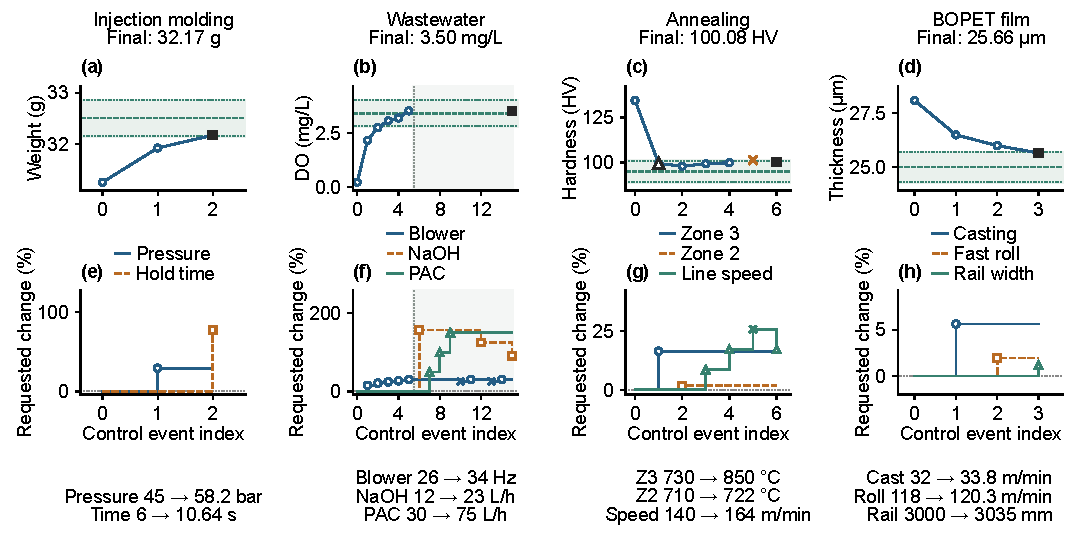
\includegraphics[width=\textwidth]{resources/fig-missions-controls.pdf}
\caption{Four-scenario simulator control sequences and outcomes (seed 42; one
scripted trajectory per scenario through the platform's governed operation
API). Upper panels show process-variable (PV) observations and scenario-specific
target windows; lower panels show requested setpoint changes from baseline.
Black squares mark mission-final readings; for injection molding and BOPET they
overlap the last observation.
In wastewater treatment, later sodium-hydroxide (NaOH) and polyaluminium-
chloride (PAC) requests belong to pH and total-phosphorus stages, and the
mission-final dissolved-oxygen (DO) reading (3.50\,mg/L) is not
joined to the last trajectory observation (3.517\,mg/L). Crosses mark reverted
requests. In annealing, Z3 and Z2 denote zone-3 and zone-2 temperature
setpoints. The open triangle marks the 99.46 Vickers-hardness (HV) event
without a linked optimization record; the cross is the
101.3-HV event-text value after a reverted 176\,m/min candidate, not a
structured
trajectory observation. Requests are not device readbacks. These scripted
scenario missions are separate from the route-continuity study and do not
establish route-level process performance or a common optimizer score.}
\label{fig:missions}
\end{figure*}

Injection-molding pressure and hold-time changes accompanied a weight increase
from 31.25 to 32.17\,g, within the $32.5\pm0.35$\,g window. Five wastewater
blower increments raised dissolved oxygen (DO) from 0.214 to 3.517\,mg/L,
within the $3.4\pm0.6$\,mg/L window; subsequent NaOH and polyaluminium
chloride (PAC) actions addressed separate pH and phosphorus stages. In
annealing, zone-3/zone-2 setpoints and line-speed changes preceded a terminal Vickers hardness of
100.08\,HV,
within the $95\pm6$\,HV window. Biaxially oriented polyethylene
terephthalate (BOPET) thickness fell from 28.10 to 25.66\,$\mu$m under the
plotted casting, roll-speed, and rail-width changes, within its
$25.0\pm0.7$\,$\mu$m window. Thus, each scripted mission reported a terminal
value in its scenario target window. Wastewater and annealing terminal values
differ from their final structured trajectory observations, as marked in
Fig.~\ref{fig:missions}. One trajectory per scene shows scenario-specific
feedback but does not establish repeatability or route-level process
attainment; the route and mission studies used different entry, controller,
and sampling protocols.
\subsection{Evidence Synthesis}
Across the studies, tested routes retained their applicable records across two
configured mappings, but all 12 route samples remained below target. The
blueprint replay completed one documented onboarding workflow and a confirmed
simulator write; the mock-state guard blocked injected stale contexts before
software dispatch. The four mission-terminal values fell within their
scenario-specific windows. These results support selected integration and
scenario-specific simulator behavior. Because entry and sampling protocols
differ, the process datasets are not pooled. Verified readback confirms the
command path, while the later sample records process status; neither establishes
route-level process attainment, repeatability, process improvement, general
portability, or physical-plant performance. Supplementary File S1 contains the
supporting evidence.
